\documentclass[12pt]{mwart}

\usepackage{polski}
\usepackage[utf8]{inputenc}
\usepackage{mathtools,icomma,graphicx,float,enumitem, bm,amsmath,amssymb, mdsymbol, textcomp, subfigure, scrextend, float, upgreek, xfrac, setspace}
\usepackage[table,xcdraw]{xcolor}
\usepackage{tabularray, tabularx}
\mathtoolsset{mathic}
\raggedbottom
\graphicspath{ {./images/} }

\author{Mateusz Stasiak \\ Indeks: 262339}
\title{Proces Ryzyka i ruch Browna}

\begin{document}
		\begin{center}
		{\Large\textbf{Symulacje Komputerowe}}
	\end{center}
	\begin{center}
		Raport: \textbf{2}
	\end{center}
	
	\noindent Temat sprawozdania  \textbf{Proces Ryzyka i ruch Browna} \\
	Nazwisko i Imię prowadzącego kurs \textbf{dr Michał Balcerek} 	\newline\newline
	
	
	\noindent\begin{tabularx}{\textwidth}{|X |X|}
		\hline
		Wykonawca: & \\\hline
		\begin{center}
			Imię i Nazwisko,\\ nr indeksu
		\end{center} &  \begin{center}
			Adrianna Ziobroniewicz, 262227\\
			Mateusz Stasiak, 262339
		\end{center}\\\hline
		Wydział & Wydział Matematyki, W13 \\\hline
		Termin zajęć: & Wtorek,\vphantom{ $11^{1^{5}}$} $11^{15}$\\\hline
		Numer grupy ćwiczeniowej & T00-70d \\\hline
		Data oddanie sprawozdania: & \today \\\hline
		\textbf{Ocena końcowa} &\\\hline
		
	\end{tabularx}\newline\newline
	
	
	\noindent\textbf{Adnotacje dotyczące wymaganych poprawek oraz daty otrzymania poprawionego sprawozdania}
	
	\newpage
	
	\begin{spacing}{2}
	\tableofcontents
	\end{spacing}
	
	\newpage
	
	
	\section{Zadanie 1}
	\subsection{Wstęp}
	\subsubsection{Proces ryzyka}
	\noindent Proces ryzyka to proces stochastyczny opisujący kapitał firmy ubezpieczeniowej na horyzoncie czasowym $T$. Zadany jest wzorem
	\begin{equation}
		R(t) = u + c(t) - \sum^{N(t)}_{i=1} X_i, \quad \mathrm{gdzie:} \label{ryzyko}
	\end{equation}
	
	\begin{enumerate}
	\itemsep 1mm
		\item $t \in [0,T]$
		\item $u > 0$ to kapitał początkowy 
		\item $c(t)$ to premia (przychody ze sprzedaży polis)
		\item $N(t)$ to proces liczący straty
		\item $X_i$ to zmienne losowe iid. reprezentujące wysokości wypłacanych odszkodowań, $\mathbb{E} X_i=\mu, X_i>0, X_i \upvDash N(t)$. 
	\end{enumerate}
	
	
	\noindent Klasyczny proces ryzyka zakłada liniowy przychód ze sprzedaży polis, tzn. $c(t)=c\cdot t$. Charakteryzuje się on również tym, że momenty wypłacania ubezpieczeń są generowane z jednorodnego procesu Poissona o intensywności $\lambda_{p}$. 
		
	\begin{figure}[H]
	\begin{center}
		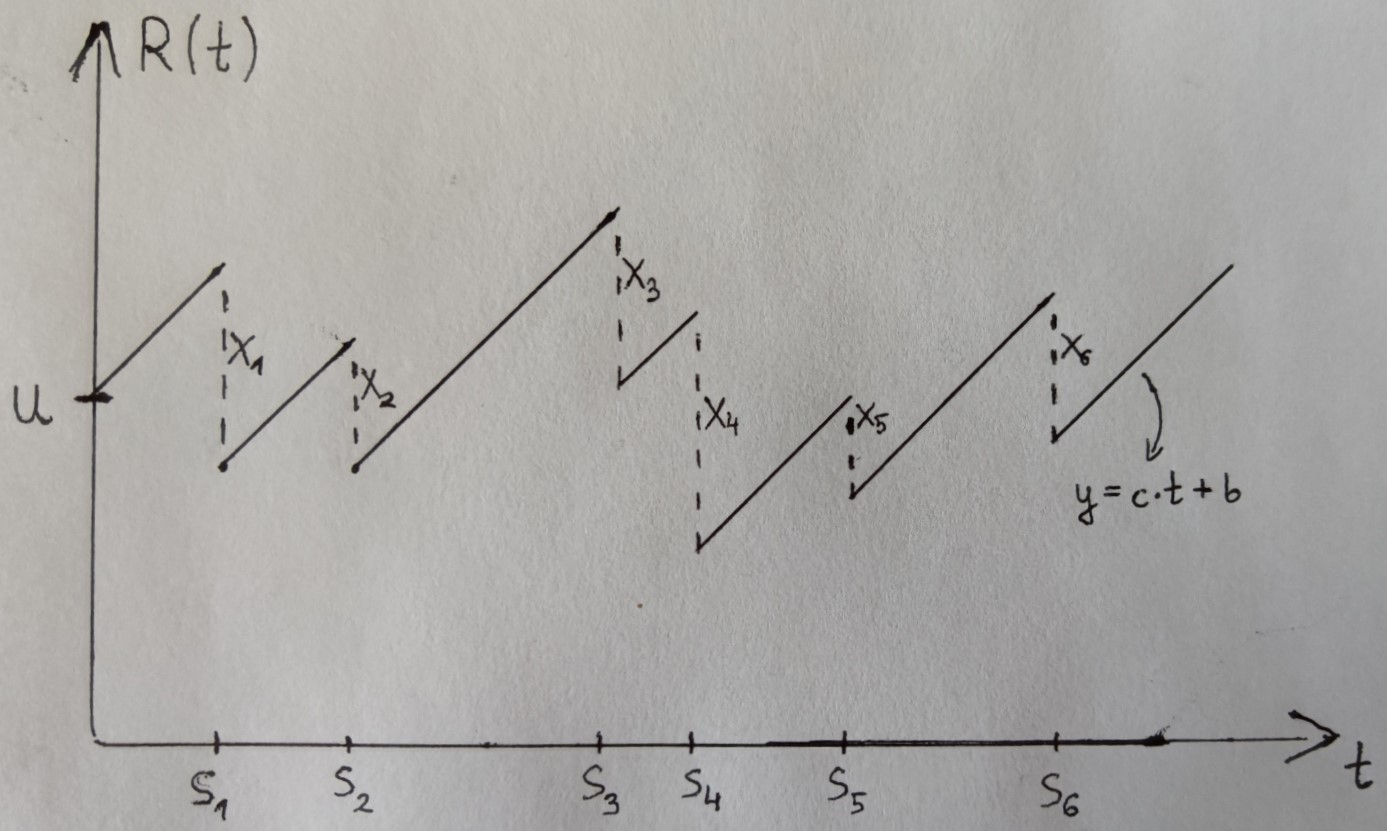
\includegraphics[scale=0.25]{proces_ryzyka.jpg}
		\caption{Klasyczny proces ryzyka (rysunek autora)}
	\end{center}
	\end{figure}
	
	
	
	
	\subsubsection{Jednorodny proces Poissona}
	\noindent Jednorodnym procesem Poissona z intensywnością $\lambda_{p}>0$ nazywamy proces liczący $\left\lbrace N(t), t \geq 0 \right\rbrace $, który spełnia następujące warunki:
	
	\begin{enumerate}
	\itemsep 1mm
		\item $N(0)=0$
		\item $N(t)$ ma niezależne i stacjonarne przyrosty
		\item $N(t) \sim Poiss(\lambda_{p} t)$, tzn. $P(N(t)=n)=e^{-\lambda_{p} t} \cdot \cfrac{(\lambda_{p} t)^{n}}{n!}$
	\end{enumerate}
	
	\noindent Zauważmy, że średnia liczba obserwacji, które pojawiły się do momentu $t$ wynosi $\mathbb{E}(N(t))=\lambda_{p} t$. Dlatego parametr $\lambda_{p}$ nazywany jest intensywnością pojawiania się zdarzeń losowych. Algorytm generowania tego procesu wygląda następująco:
	
	\begin{enumerate}
	\itemsep 1mm
		\item Tworzymy zmienną $S=0$.
		\item Generujemy $t_i \sim Exp(\lambda_{p})$. Jest to czas oczekiwania na $i$-ty skok.
		\item Jeśli $S+t_i<T$ to dodajemy wartość $t_i$ do $S$ i wracamy do punktu 2. Jeśli nie, kończymy algorytm.
		\item Kolejne wartości $S$ są wartościami jednorodnego procesu Poissona, które reprezentują momenty skoków.
	\end{enumerate}
	
	\begin{figure}[H]
	\begin{center}
		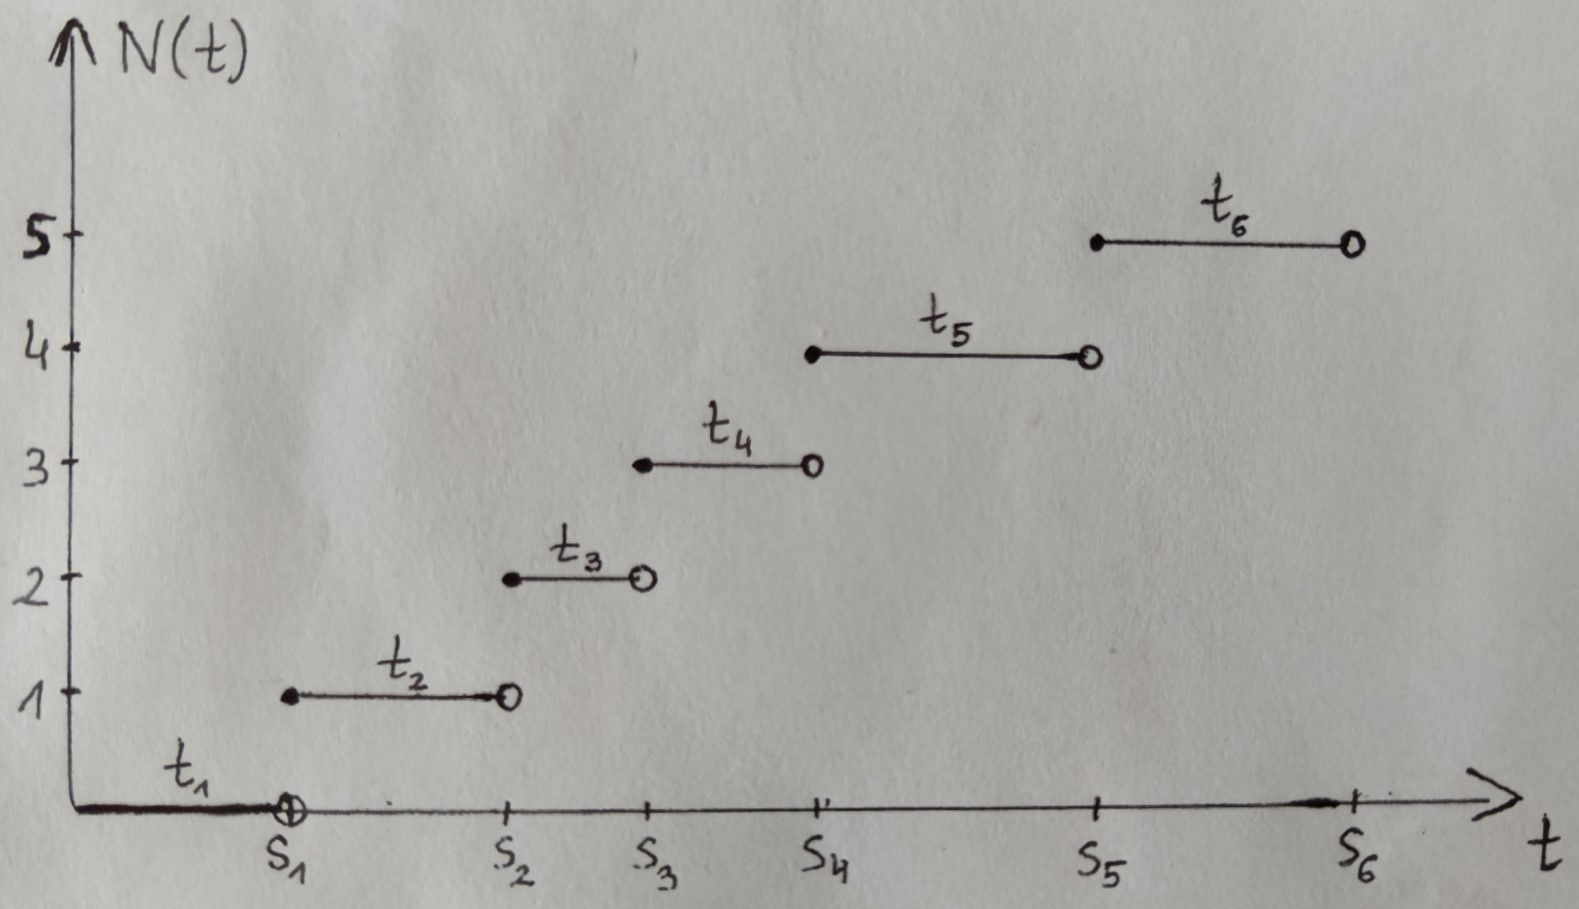
\includegraphics[scale=0.25]{proces_poissona.jpg}
		\caption{Jednorodny proces Poissona (rysunek autora)}
	\end{center}
	\end{figure}
	
	
	
	\subsection{Dane do zadania}
	\noindent W tym zadaniu pracujemy na danych otrzymanych od prowadzącego. Plik zawiera 50 trajektorii pewnego procesu ryzyka, który został wysymulowany na odcinku $[0, 100]$, z krokiem czasowym $h = 0.01$. Kapitał początkowy to $u=50$. Plik ma rozszerzenie $.p$, zatem możemy go wczytać używając języka programowania Python za pomocą polecenia pickle.load(open(\textquotesingle ŚcieżkaDoPliku\textquotesingle ,\textquotesingle rb\textquotesingle)).
	
	\begin{figure}[H]
	\begin{center}
		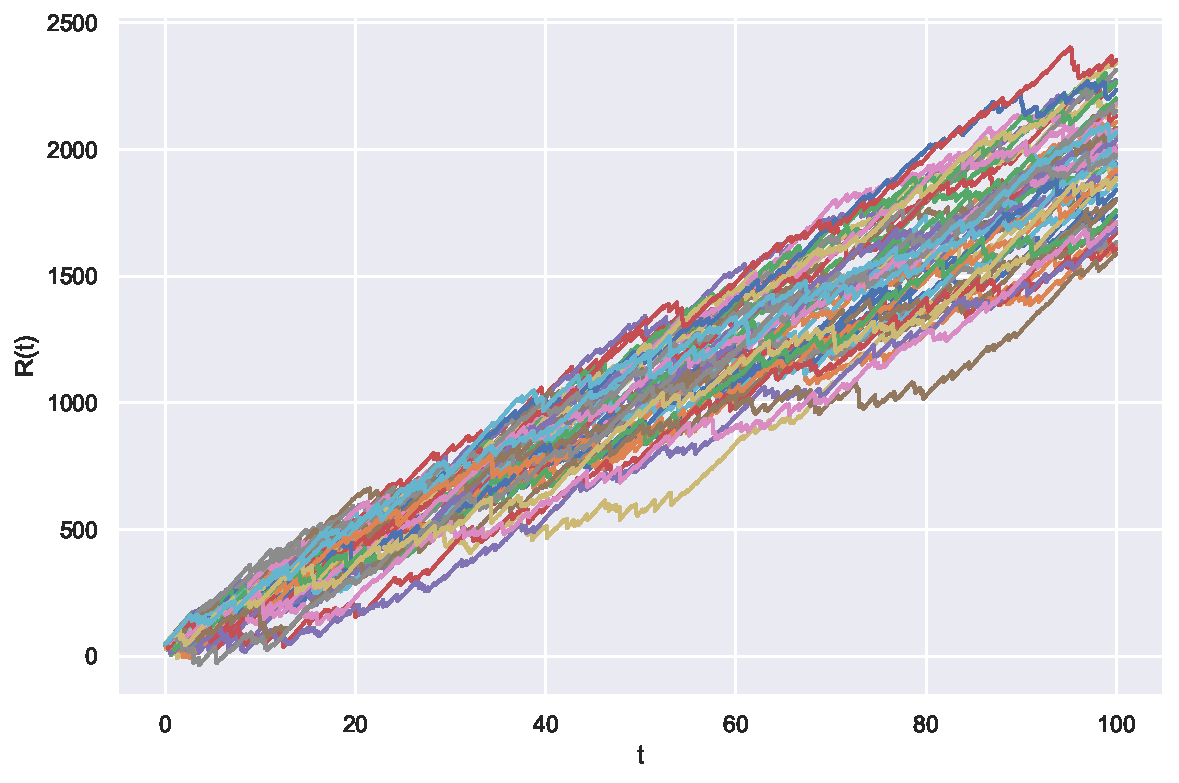
\includegraphics[scale=0.5]{dane.pdf}
		\caption{Otrzymane $50$ trajektorii procesu ryzyka}
	\end{center}
	\end{figure}
	
	\subsection{Dopasowanie klasycznego modelu ryzyka do danych}
	\subsubsection{Koszt polisy}
	\noindent Cenę ubezpieczenia możemy prosto wyznaczyć porównując ze sobą dwa pierwsze elementy każdej trajektorii. Uzasadnia to fakt, że kupienie polisy jest niezbędne, aby później klient mógł otrzymać odszkodowanie. 
	
	\begin{figure}[H]
	\begin{center}
		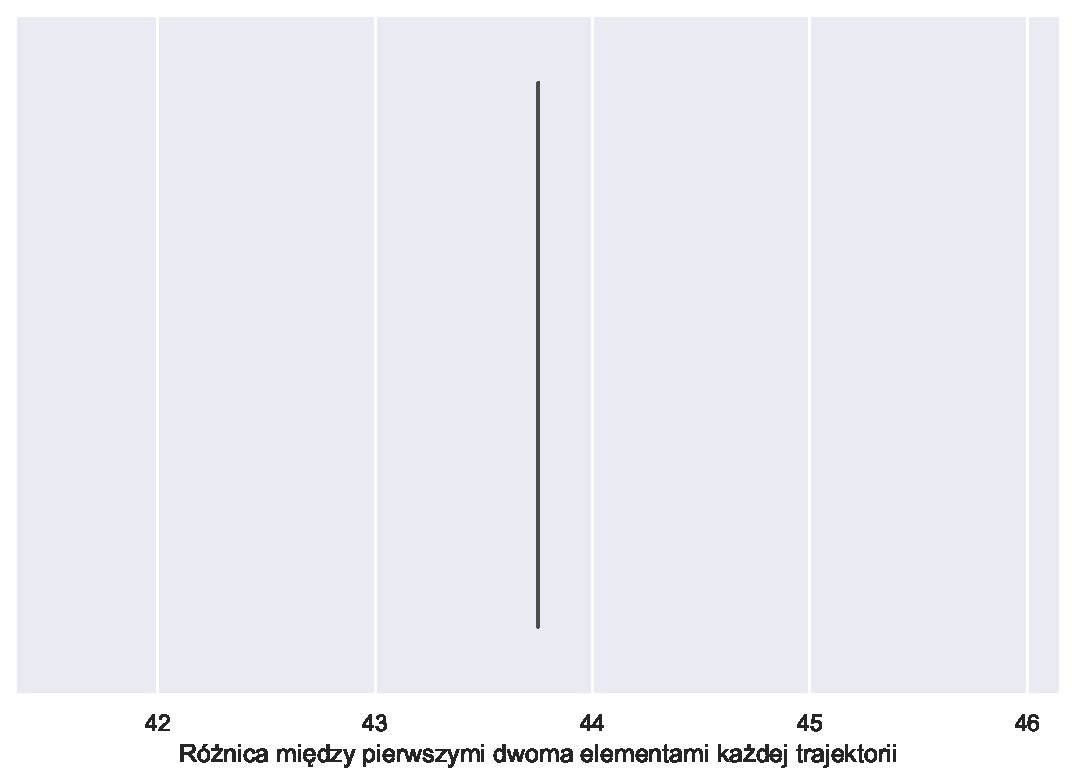
\includegraphics[scale=0.5]{box1.pdf}
		\caption{Wykres pudełkowy różnic między pierwszymi dwoma elementami \newline każdej trajektorii}
	\end{center}
	\end{figure}
	
	\noindent Dla otrzymanych danych, wszystkie trajektorie mają wspomniany przychód równy $0.4375$. Jako że elementy są od siebie oddalone o czas $h=0.01$, to przyjmujemy premię $c=43.75$.
	
	\subsubsection{Rozkład wysokości wypłacanych odszkodowań $\bm{X_i}$}
	\noindent Aby dopasować klasyczny model ryzyka do powyższych danych, należy znaleźć rozkład zmiennej losowej $X_i$, która wyznacza wartość $i$-tej szkody (wypłaconego odszkodowania). Rozkład $X_i$ jest taki sam dla każdej z trajektorii. Dlatego najłatwiej będzie wyodrębnić wszystkie spadki z otrzymanych danych, narysować ich histogram, a następnie przy pomocy gęstości empirycznej i wykresu typu QQ-plot odczytać typ i parametry gęstości rozkładu $X_i$. \\
	
	\noindent Wysokości wypłacanych odszkodowań obliczamy porównując ze sobą wartości sąsiadujących elementów każdej trajektorii. Przypomnijmy, że owe punkty są rozmieszczone co $h=0.01$, a kapitał firmy rośnie poprzez liniowy przychód ze sprzedaży polis. Dlatego jeśli różnica między dwoma sąsiadującymi punktami wynosi $c\cdot 0.01$, to w danym momencie nie nastąpiło wypłacenie odszkodowania. W innym wypadku, należy policzyć różnicę między wartością uwzględniającą sam przychód a rzeczywistym kapitałem. \\
	
	
	\begin{figure}[H]
	\begin{center}
		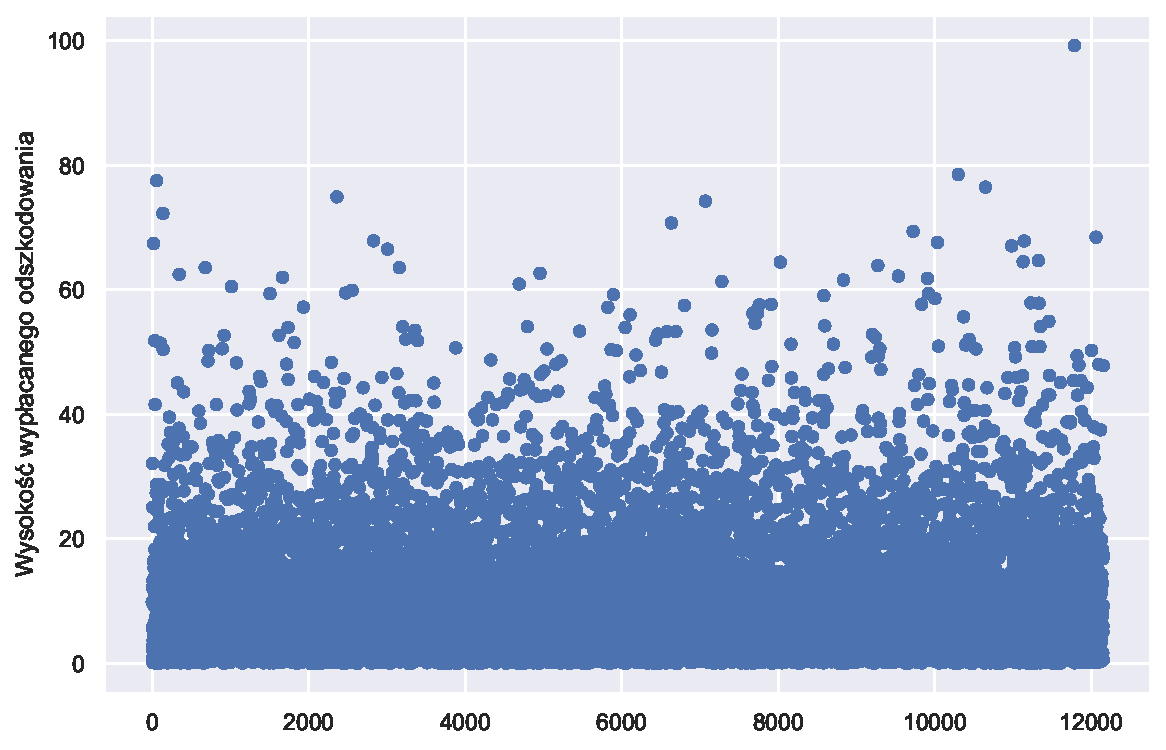
\includegraphics[scale=0.5]{scatter1.pdf}
		\caption{Wykres punktowy wartości wypłacanych odszkodowań $X_i$}
	\end{center}
	\end{figure}
	
	\begin{figure}[H]
	\begin{center}
		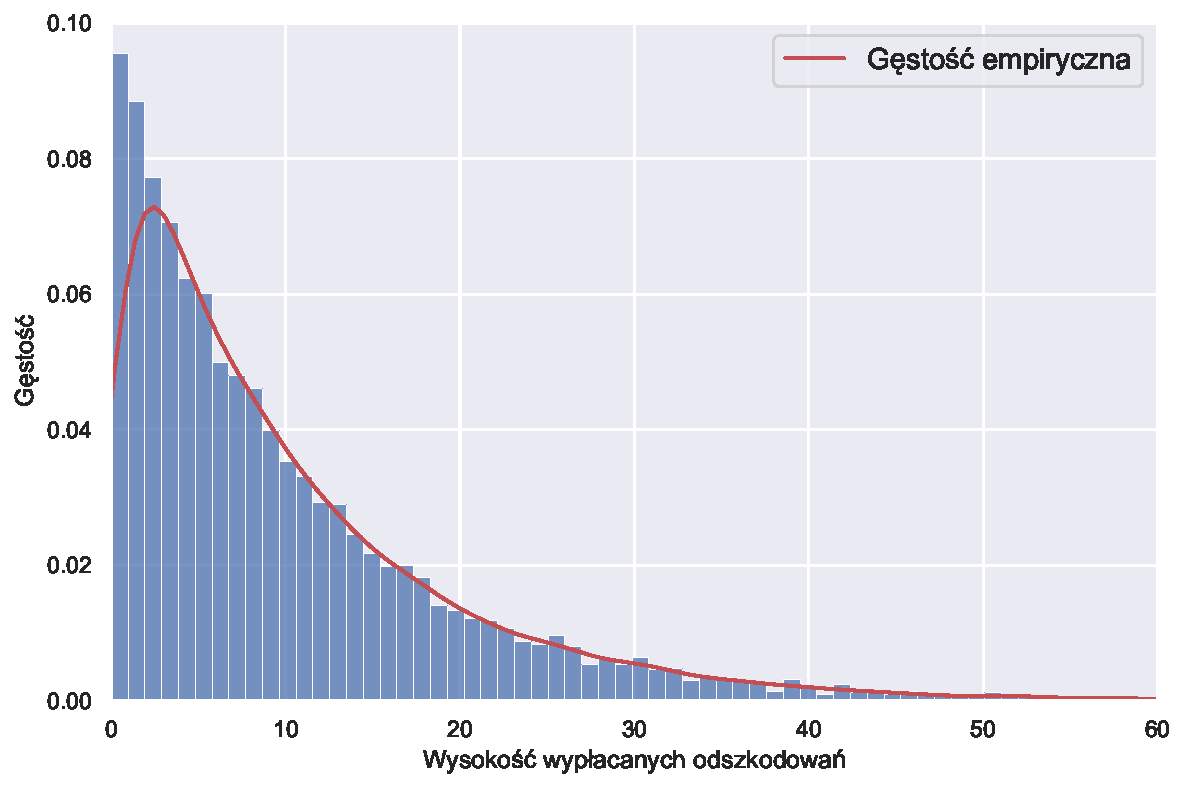
\includegraphics[scale=0.5]{histogram1.pdf}
		\caption{Histogram wartości wypłacanych odszkodowań $X_i$}
	\end{center}
	\end{figure}
	
	\noindent Zauważmy, że histogram ma kształt typowy dla rozkładu wykładniczego. Zweryfikujemy tę hipotezę poprzez wyliczenie potencjalnego parametru $\lambda_{x}$, a następnie porównanie empirycznej dystrybuanty i wykresu kwantylowego z wartościami teoretycznymi. Przypomnijmy, że dla rozkładu wykładniczego $\frac{1}{\lambda_{x}}=\mathbb{E} X_i = \overline{X} = 10.119 = \frac{1}{0.0988}$.
	
	\begin{figure}[H]
	\begin{center}
		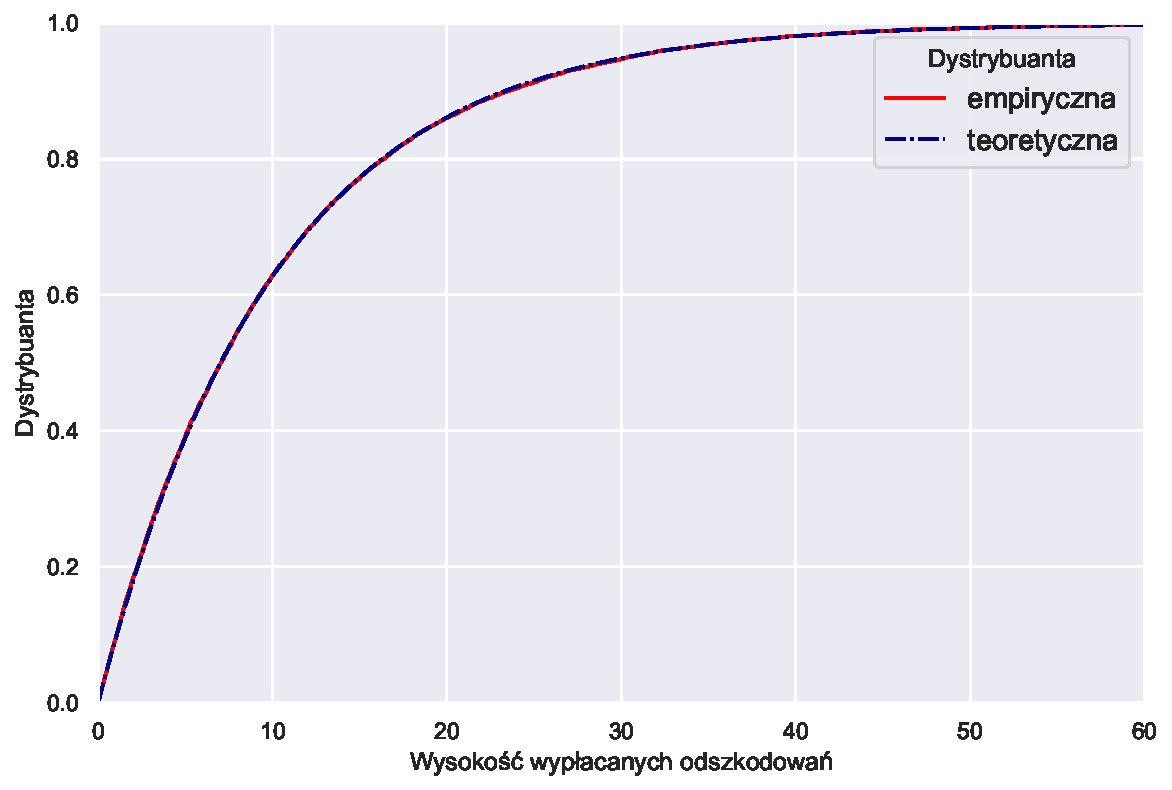
\includegraphics[scale=0.5]{dystrybuanta1.pdf}
		\caption{Porównanie dystrybuanty empirycznej z teoretyczną dla rozkładu $Exp(0.0988)$}
	\end{center}
	\end{figure}
	
	
	\begin{figure}[H]
	\begin{center}
		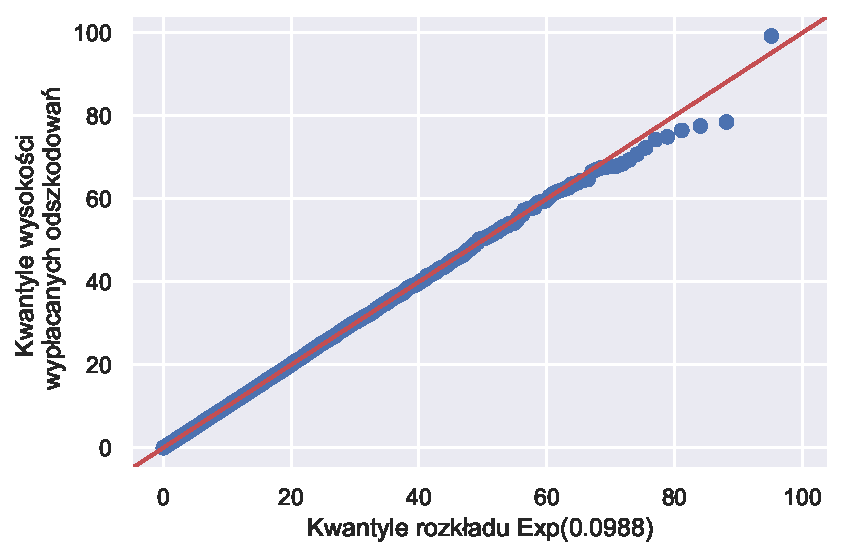
\includegraphics[scale=0.7]{qqplot1.pdf}
		\caption{Wykres kwantylowy dla wartości wypłacanych odszkodowań z argumentem $Exp(0.0988)$}
	\end{center}
	\end{figure}
	
	\noindent Dystrybuanty pokrywają się, a wykres kwantylowy stanowi linię prostą nachyloną do osi $OX$ pod kątem $45$ stopni. Oznacza to, że prawidłowo dopasowaliśmy rozkład zmiennej losowej $X_i \sim Exp(0.0988)$.
	
	
	
	\subsubsection{Intensywność wypłacania ubezpieczeń}
	\noindent Kolejnym krokiem jest wyznaczenie intensywności wypłacania ubezpieczeń. Inaczej mówiąc, musimy znaleźć parametr $\lambda_{p}$ jednorodnego procesu Poissona. W tym celu znajdziemy momenty pojawienia się spadków kapitału. Następnie wyliczymy czasy oczekiwania na kolejne skoki. Przy pomocy histogramu, dystrybuanty empirycznej i wykresu kwantylowego zbadamy rozkład tych zmiennych losowych. Ze względu, że jest to klasyczny model ryzyka, parametr tego rozkładu będzie odpowiadał $\lambda_{p}$ w jednorodnym procesie Poissona.
	
	
	\begin{figure}[H]
	\begin{center}
		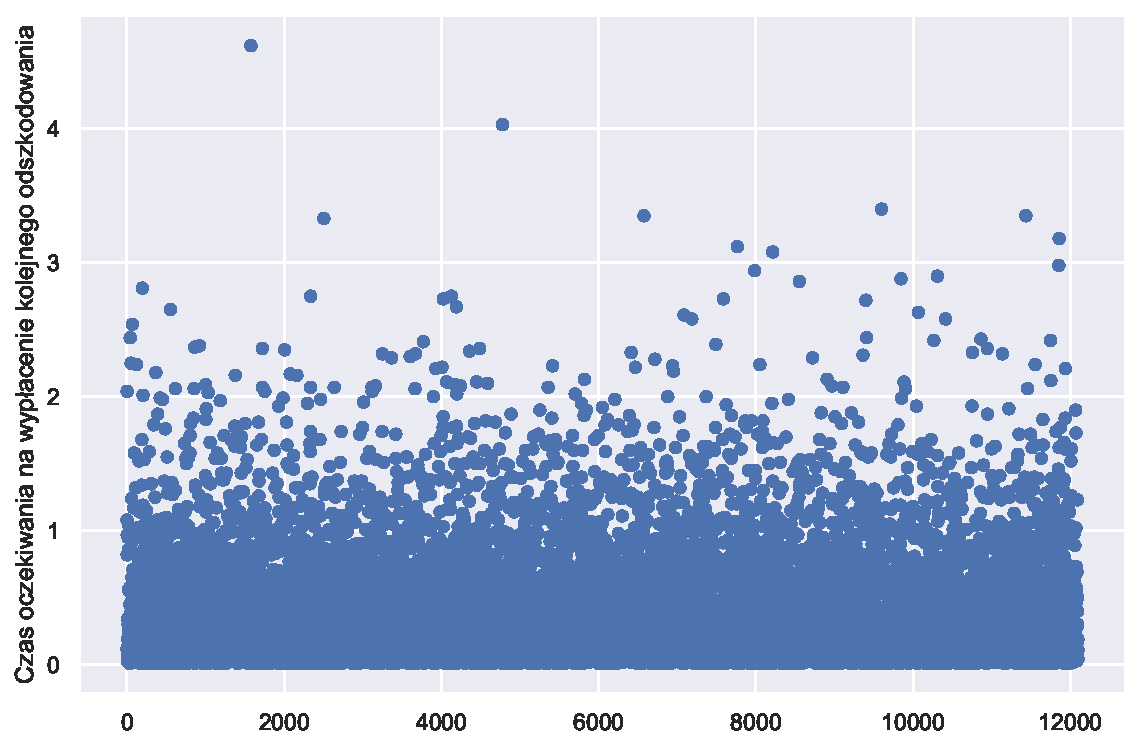
\includegraphics[scale=0.5]{scatter2.pdf}
		\caption{Wykres punktowy czasów oczekiwania na wypłacenie \newline kolejnego odszkodowania}
	\end{center}
	\end{figure}
	
	\begin{figure}[H]
	\begin{center}
		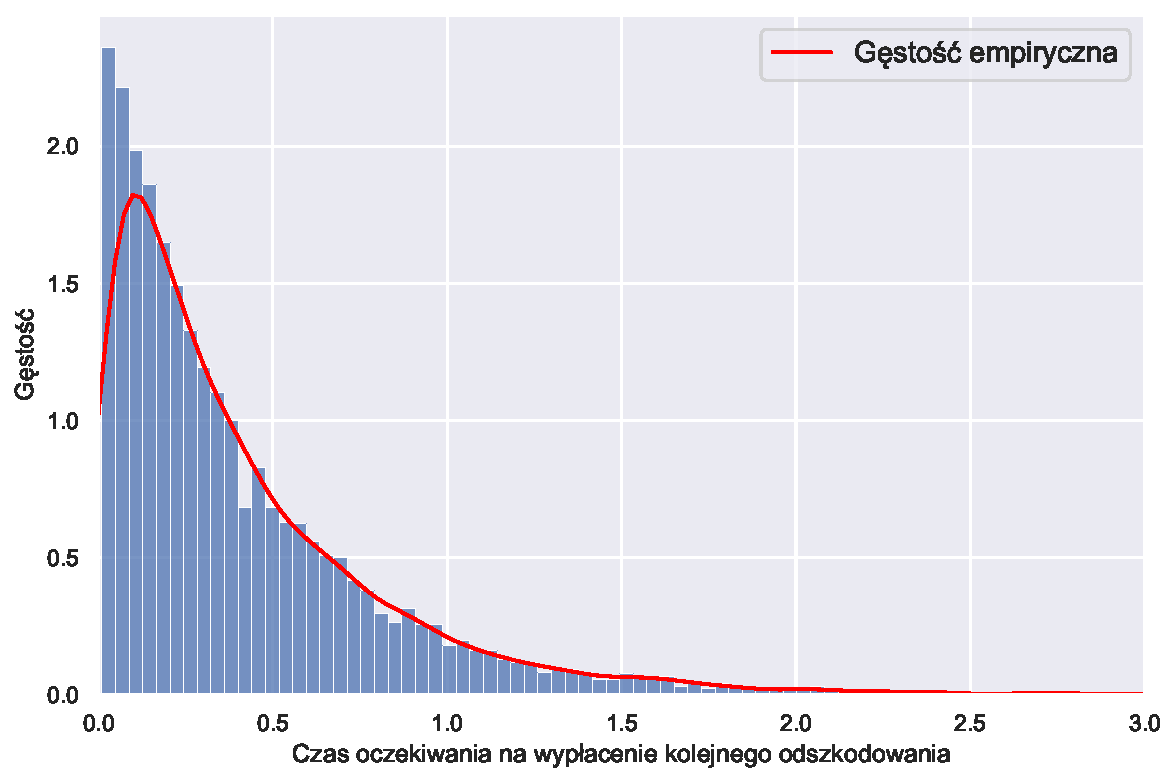
\includegraphics[scale=0.5]{histogram2.pdf}
		\caption{Histogram czasów oczekiwania na wypłacenie \newline kolejnego odszkodowania}
	\end{center}
	\end{figure}
	
	\noindent Zauważmy, że histogram ma kształt typowy dla rozkładu wykładniczego. Zweryfikujemy tę hipotezę poprzez wyliczenie potencjalnego parametru $\lambda_{p}$, a następnie porównanie empirycznej dystrybuanty i wykresu kwantylowego z wartościami teoretycznymi. Przypomnijmy, że dla rozkładu wykładniczego $\frac{1}{\lambda_{p}}=\mathbb{E} t_i = \overline{t} = 0.41 = \frac{1}{0.41}$.
	
	
	\begin{figure}[H]
	\begin{center}
		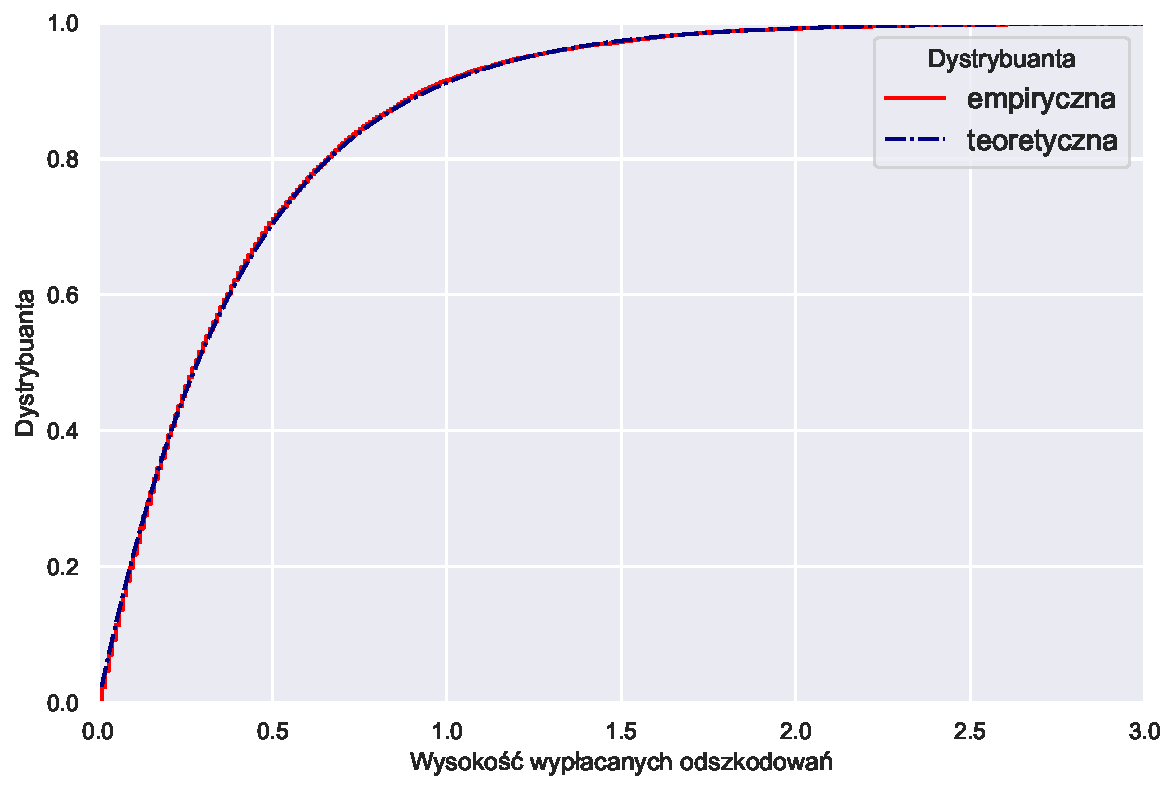
\includegraphics[scale=0.5]{dystrybuanta2.pdf}
		\caption{Porównanie dystrybuanty empirycznej z teoretyczną dla rozkładu $Exp(2.4388)$}
	\end{center}
	\end{figure}
	
	
	\begin{figure}[H]
	\begin{center}
		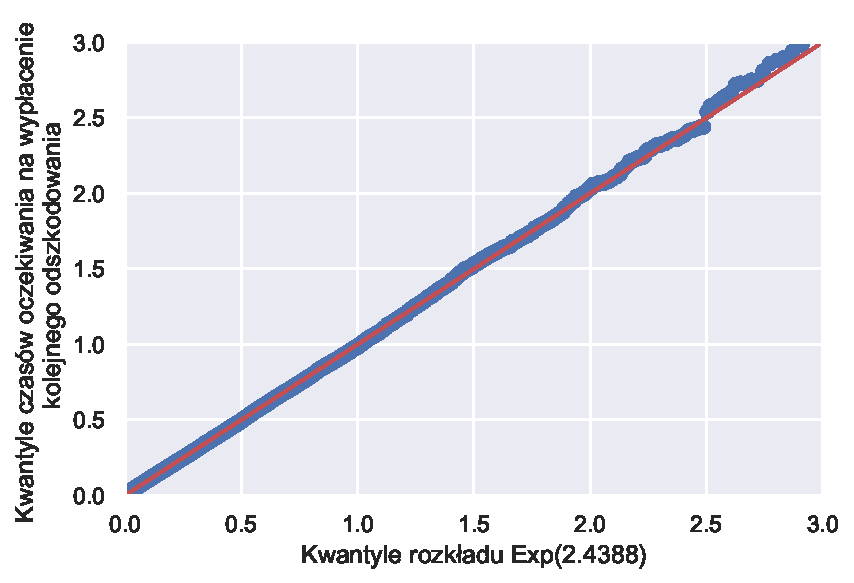
\includegraphics[scale=0.7]{qqplot2.pdf}
		\caption{Wykres kwantylowy dla czasów oczekiwania na wypłacenie kolejnego odszkodowania z argumentem $Exp(2.4388)$}
	\end{center}
	\end{figure}
	
	\noindent Dystrybuanty pokrywają się, a wykres kwantylowy stanowi linię prostą nachyloną do osi $OX$ pod kątem $45$ stopni. Oznacza to, że prawidłowo dopasowaliśmy rozkład zmiennej losowej $t_i$. Czasy oczekiwania na wypłacenie kolejnego odszkodowania są z rozkładu $Exp(2.4388)$, zatem nasz proces liczący (jednorodny proces Poissona) przyjmuje parametr intensywności $\lambda_{p} = 2.4388$. 
	
	
	\subsubsection{Bezpieczeństwo firmy} \label{theta}
	\noindent Bezpieczeństwo finansowe stanowi priorytet każdej firmy. Dlatego wysokość ceny polisy jest determinowana przez tzw. narzut bezpieczeństwa $\theta$ zgodnie ze wzorem $c=(1+\theta)\lambda_{p} \mathbb{E} X_i$. Obliczmy narzut dla otrzymanych danych:
	$$\theta = \frac{c}{(\mathbb{E} X_i) \cdot \lambda_{p}} - 1 = 0.7728.
	$$
	
	\subsection{Wnioski}
	\noindent W tej części zadania udało nam się dopasować klasyczny model ryzyka do otrzymanych danych. Ustaliliśmy, że premia $c=43.75$, wysokości odszkodowań $X_i$ mają rozkład $Exp(0.0988)$, a intensywność wypłacania ubezpieczeń wynosi $\lambda_{p} = 2.4388$. Wysoka wartość parametru $\theta = 0.7728$ pozwala przypuszczać, że procesy ryzyka symulowane w drugiej części zadania rzadko kiedy zakończą się bankructwem.
	
	
	\section{Symulacje procesu ryzyka}
	\noindent Ta część zadania polega na wysymulowaniu $100$ trajektorii klasycznego procesu ryzyka $R(t)$ z parametrami obliczonymi w poprzedniej sekcji. Następnie zajmiemy się analizą stworzonych danych pod kątem bankructwa. Algorytm symulacji przebiega następująco:
	
	\begin{enumerate}
		\item Generujemy jednorodny proces Poissona $N(t)$ na $[0,T]$. Czasy oczekiwania na kolejne spadki mają rozkład $Exp(2.4388)$.
		\item Generujemy $X_1, X_2, \ldots, X_{N(t)}$. Wysokości spadków mają rozkład $Exp(0.0988)$.
		\item Ustalamy początkowy kapitał $u$ i podstawiamy wartości do wzoru numer \ref{ryzyko} na stronie \pageref{ryzyko}.
	\end{enumerate}
	
	\noindent Otrzymaną wiązkę zestawiamy na wykresie ze średnią procesu oraz jedną trajektorią z pliku z danymi.
	
	\begin{figure}[H]
	\begin{center}
		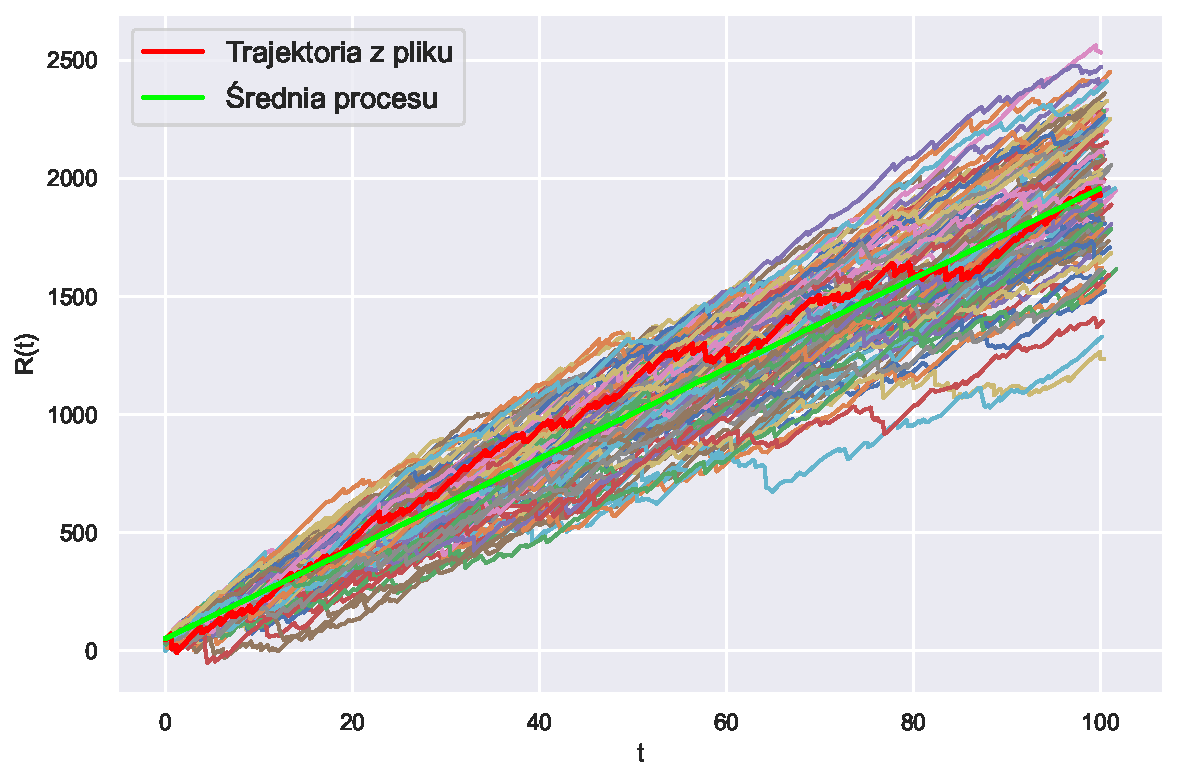
\includegraphics[scale=0.5]{symulacja1.pdf}
		\caption{Porównanie 100 wysymulowanych trajektorii $R(t)$ ze średnią procesu oraz jedną trajektorią z pliku}
	\end{center}
	\end{figure}
	
	\noindent Czerwona i zielona trajektoria biegną przez wygenerowaną wiązkę klasycznego procesu ryzyka. Świadczy to o poprawności wykonanej przez nas symulacji.
	
	
	
	\subsection{Definicja bankructwa}
	\noindent Bankructwo to moment, w którym wartość procesu ryzyka $R(t)$ pierwszy raz spadnie poniżej zera. Możemy go zapisać w postaci:
	$$\tau(u) \overset{\mathrm{def}}{=} \text{inf} \{t \geq 0: R(t) <0\}.$$
	
	
	\subsection{Prawdopodobieństwo ruiny dla skończonego horyzontu czasowego}
	\noindent Rozpatrując skończony horyzont czasowy, możemy policzyć prawdopodobieństwo, że firma zbankrutuje do pewnego momentu $T$:
	$$\Psi (u,T) \overset{\mathrm{def}}{=} P \left(   \tau (u) < T \right) .
	$$
	\noindent Jedną z metod wyznaczenia powyższego prawdopodobieństwa jest metoda Monte Carlo. Algorytm działania wygląda następująco:
	\begin{enumerate}
	\itemsep 2mm
		\item Generujemy $N$ trajektorii procesu ryzyka $R_1(t), \ldots , R_N(t)$ na przedziale $[0,T]$.
		\item Wyznaczamy liczbę trajektorii $n$, które spadły poniżej zera na przedziale $[0,T]$. $\ n=\#\left\lbrace i \in \left\lbrace 1, \dots , N \right\rbrace \colon \mathrm{min}\ R_i(t) < 0 \right\rbrace $. 
		\item Podstawiamy do wzoru $\Psi (u,T)=\frac{n}{N}$. \\
	\end{enumerate}
	
	\noindent Po przeprowadzeniu symulacji Monte Carlo otrzymaliśmy wyniki $\Psi (50,100)= 0.065$ oraz $\Psi (50,200)= 0.0691$. Oznacza to, że zaledwie kilka procent trajektorii kończy się bankructwem. Zgadza się to z wysoką wartością parametru $\theta$ w sekcji \ref{theta}.
	
	
	\subsection{Prawdopodobieństwo ruiny dla nieskończonego horyzontu czasowego}
	\noindent Rozpatrując nieskończony horyzont czasowy, możemy policzyć prawdopodobieństwo, że firma kiedykolwiek zbankrutuje. W tym przypadku nie ustalamy konkretnego przedziału czasowego, więc wzór nie zależy od $T$:
	$$\Psi (u) \overset{\mathrm{def}}{=} P \left(   \tau \left( u \right) < \infty \right). 
	$$
	
	\noindent Powyższe prawdopodobieństwo możemy aproksymować za pomocą wzoru Pollaczka-Chinczyna o postaci:
	$$\Psi (u) = \frac{\theta}{1+\theta} \sum^{\infty}_{n=0} (\frac{1}{1+\theta})^n B_n(u), \quad \mathrm{gdzie:}
	$$
	\begin{itemize}
	\itemsep 1mm
		\item [$\bullet$] $B_n(u) = P(Y_1 + \ldots + Y_n > u)$
		\item [$\bullet$] $Y_i$ to zmienne losowe iid. o gęstości $f(x) \overset{\mathrm{def}}{=} \frac{1-F_{X_i}(x)}{\mu}, \quad \mathrm{gdzie} \quad \mu=\mathbb{E} X_i$.
	\end{itemize}
	
	\noindent Wyznaczanie prawdopodobieństwa ruiny $\Psi (u)$ dla nieskończonego horyzontu czasowego za pomocą metody Monte Carlo ma następujący algorytm:
	
	\begin{enumerate}
	\itemsep 2mm
		\item Tworzymy tablicę $Z$ o rozmiarze $N$.
		\item Generujemy zmienną losową $K \sim Geom(\frac{\theta}{1+\theta})$.
		\item Generujemy zmienne losowe iid. $Y_1, \ldots , Y_K$, każda z nich o gęstości $f(x)=\frac{1-F_{X_i}(x)}{\mu}$.
		\item Jeśli $Y_1 + \ldots + Y_K > u$ wstawiamy $Z[i] = 1$, w przeciwnym razie $Z[i]=0$.
		\item Powtarzamy $N$ razy kroki od 2 do 4.
		\item Podstawiamy do wzoru $\Psi (u)=\frac{Z[1]+\ldots +Z[N]}{N}.$
	\end{enumerate}
	
	\noindent Po przeprowadzeniu symulacji Monte Carlo otrzymaliśmy wynik $\Psi (50)=0.06809$. Niskie prawdopodobieństwo ruiny ponownie zgadza się z wysoką wartością parametru $\theta$ w sekcji \ref{theta}. \\
	
	\noindent Przypomnijmy, że wysokości wypłacanych odszkodowań pochodzą z rozkładu wykładniczego. Pozwala to na obliczenie wartości teoretycznej prawdopodobieństwa ruiny przy nieskończonym horyzoncie czasowym. Analityczny wzór dany jest wzorem:
	$$\Psi (u)=\cfrac{1}{1+\theta} \cdot \exp \left( -\lambda_X u \cdot \frac{\theta}{1+\theta} \right) 
	$$
	
	\noindent Podstawiając $u=43.75$, $\theta=0.7728$, $\lambda_X=0.0988$ otrzymujemy $\Psi (50)=0.0654$.
	
	\subsection{Wnioski}
	\noindent Dzięki parametrom wyliczonym w pierwszej części zadania udało się nam przeprowadzić symulacje klasycznego procesu ryzyka. Wygenerowane trajektorie pasują do tych otrzymanych od prowadzącego. Następnie wyznaczyliśmy prawdopodobieństwo bankructwa dla omawianego klasycznego modelu ryzyka. Rząd tych wartości zgadza się z naszymi oczekiwaniami względem parametru $\theta$. Co więcej, wykazaliśmy niewielką różnicę między prawdopodobieństwem ruiny dla horyzontu $T=100$ i $T=200$. Oczywiście, dwie obserwacje to za mało, by wyciągnąć jakieś wnioski. Mimo to, wstępnie możemy założyć, że dla wysokich wartości parametru $\theta$, długość horyzontu nie ma wpływu na prawdopodobieństwo ruiny. Rozpatrując nieskończony horyzont czasowy porównaliśmy wzór analityczny z aproksymacją Pollaczka-Chinczyna. Mała rozbieżność wyników potwierdza prawidłowe przeprowadzenie symulacji procesu ryzyka.
	
	
	\section{Zadanie 2}
	\subsection{Ruch Browna, inaczej proces Wienera}
	\noindent Ruch Browna należy do procesów H - samopodobnych. Mówimy o~procesie~Wienera, gdy\\
	1. B(0)=0\\
	2. B(t) ma niezależne, stacjonarne przyrosty.\\
	3. $B(t) \sim N(0,t)$\\
	4. B(t) ma ciągłe trajektorie.\\
	B(t) jest $\frac{1}{2}$ - samopodobny, $B(at)=a^{\frac{1}{2}}B(t)$, $H=\frac{1}{2}$.\\
	\newline
	\noindent\textbf{Symulacja trajektorii B(t)}\\
	\noindent\textbf{Cel}: Chcemy wygenerować trajektorię B(t) w punktach $t_0, t_1,...,t_n$, gdzie $t_i=ih$, $h=\frac{1}{n}$, i=0,1,...,n.\\ Chcemy wygenerować wektor $(B(t_0),B(t_1),...,B(t_n))$. Zauważmy, że \\ $B(t_k)-B(t_{k-1})\stackrel{d}=B(t_k-t_{k-1})=B(h)$. Zatem wystarczy generować przyrosty B(t).\\
	\\
	Ruch Browna nazywany jest również procesem gaussowskim. \\ \\
	\noindent\textbf{\textit{Algorytm}}
	\begin{enumerate}
		\item[1.] $B(t_0)=0,\ (t_0=0)$
		\item[2.] $B(t_{i+1})=B(t_i)+h^{\frac{1}{2}} \xi_i$, i=0,1,...,n-1,\\ $\xi_0,...,\xi_{n-1} - iid$, $\xi_i \sim N(0,1)$, \\$h^{\frac{1}{2}}\xi_i \sim N(0,h)$
	\end{enumerate}
	
		\begin{figure}[H]
		\begin{center}
			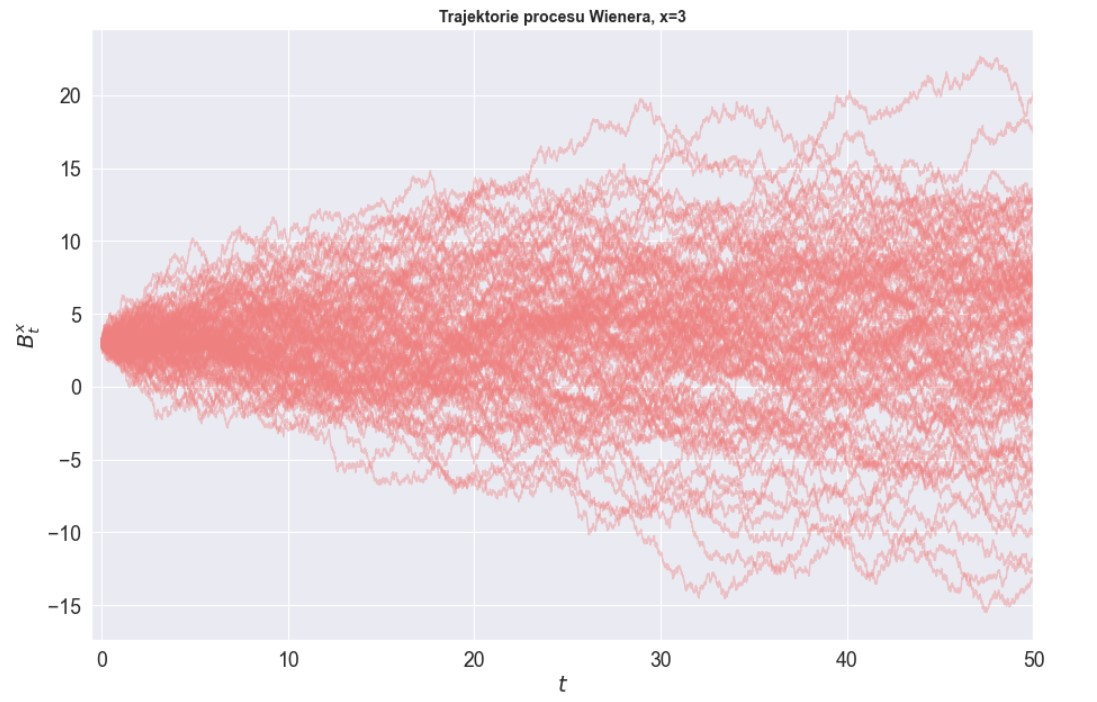
\includegraphics[scale=0.4]{trajektoria.jpg}
			\caption{Trajektoria procesu Wienera}
		\end{center}
	\end{figure}
	
	\noindent Ze wzoru $\sqrt{2t \log(\log t)}$, gdzie $t = 50$, otrzymujemy wynik w przybliżeniu $\approx 11.68$. Możemy zobaczyć, że nasze trajektorie oscylują właśnie pomiędzy asymptotami wyliczonymi ze wzorów $\sqrt{2t\log(\log t)}$ oraz $-\sqrt{2t\log(\log t)}$.\\
	
	\noindent Własności trajektorii:\\
	1. ciągłe\\
	2. nieróżniczkowalne\\
	3. niekończące wahania na zadanym odcinku.\\
	\\ \\ \\
 Funkcja gęstości ruchu Browna prezentuje się w następujący sposób:\\
 \begin{figure}[H]
 	\begin{center}
 		
 		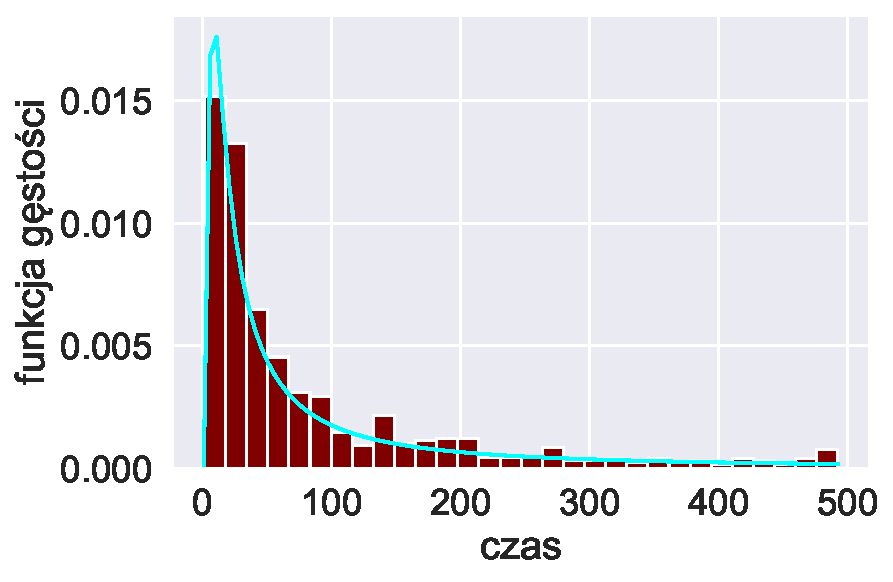
\includegraphics[scale=0.7]{gestosc.pdf}
 		\caption{Funkcja gęstości wyznaczona dla procesu Wienera}
 	\end{center}
 \end{figure}
	
	
	\subsubsection{Średni czas wyjścia z przedziału $\bm{[a,b]}$}
	\noindent Dla procesu $B_{t}^0$ bez przesunięcia o $x$ możemy definiować czas pierwszego uderzenia w ustalonym punkcie $a$:
	
		$$\tau^x=\inf\left\{t\geqslant0:B^x_t=a \right\}.$$
	
	 \noindent Dla przesunięcia:\\
	 Niech $\left\{B^x_t\right\}_{t\geqslant0}$ będzie ruchem Browna startującym z $x\in\mathbb{R}$, a $\tau^x$ czasem wyjścia tego procesu z ustalonego przedziału $[a, b]$, czyli

		$$\tau^x=\inf\left\{t\geqslant0:B^x_t\notin[a, b]\right\}.$$
	
\noindent Tutaj przyjęliśmy $b = -a$, a jeśli przyjmiemy $x \in [a,b]$, to przesuwanie o tą stałą nie zmieni naszego wyniku końcowego. Parametr $b = 5$, został wybrany tak aby wartości mniejsze od $\sqrt{2t\log(\log(t))} \approx 11,68$ były na pewno w takim czasie przyjmowane, przyjęliśmy $t=50$, dla $x=2$. 
Można pokazać, że $E\tau^x < \infty$. Dodatkowo wiemy, że średnia w próbie jest dobrym estymatorem wartości oczekiwanej.
Estymacja czasów wyjścia trajektorii poza przedział była przeprowadzana za pomocą symulacji Monte Carlo (algorytmem dla uśredniania czasów, a nie binarnych wartości).

	\begin{figure}[H]
		\begin{center}
			
			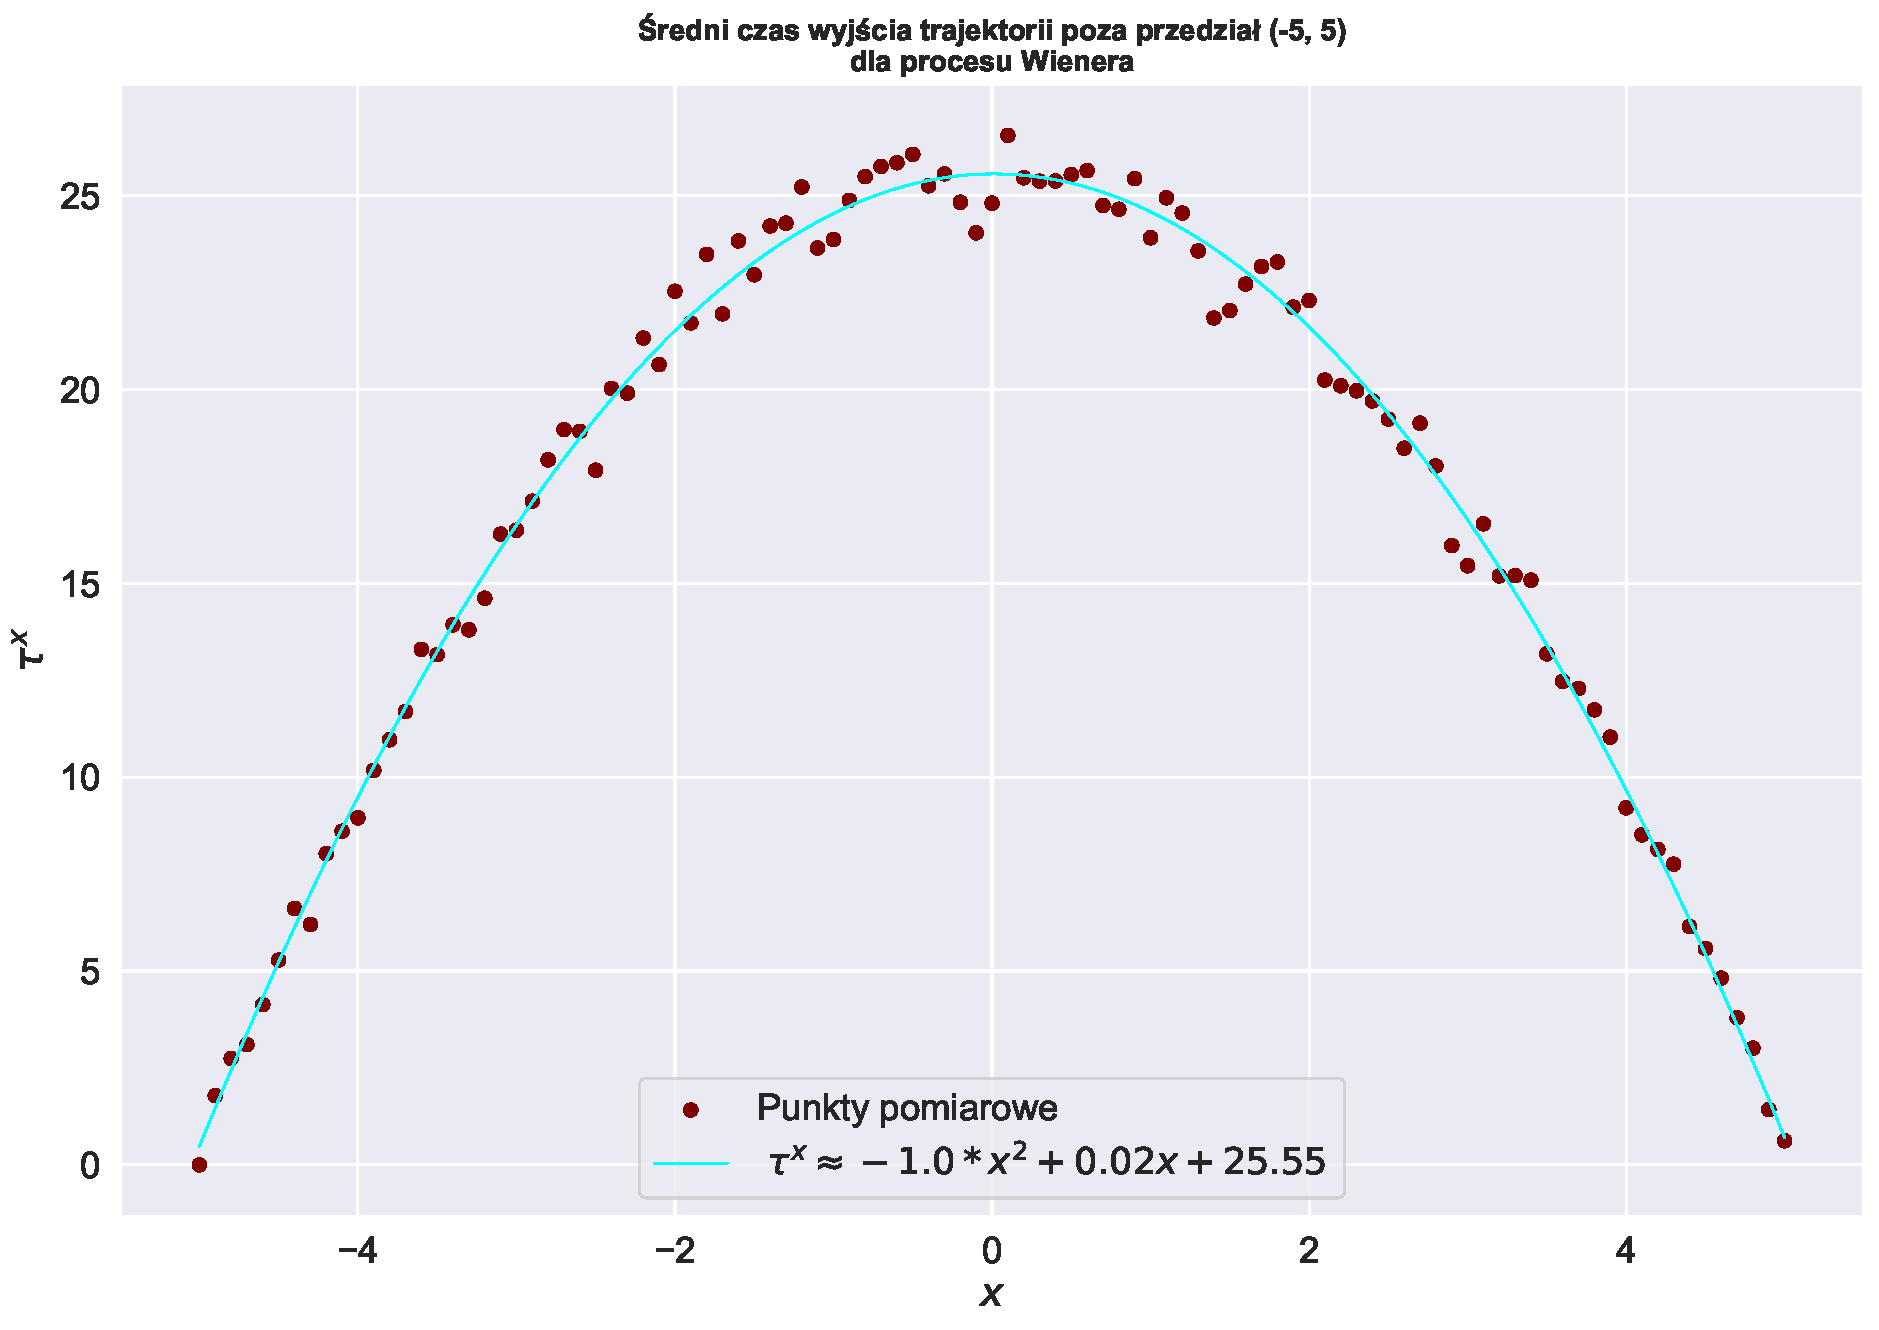
\includegraphics[scale=0.4]{1.pdf}
			\caption{Średni czas wyjścia z zadanego przedziału dla procesu Wienera \newline wraz z krzywą dopasowania.}
		\end{center}
	\end{figure}
	\noindent Wyniki symulacji zaprezentowane na tym rysunku pokazują nam, że punkty pomiarowe kształtem przypominają parabolę. Prawdą jest, że w środku przedziału czas musi być najdłuższy, gdyż tutaj wariancja rośnie razem z czasem. Symetryczność wykresu wynika z rozkładu normalnego, który charakteryzuje ruch Browna.
	Mogliśmy podejrzewać, że nasz wykres będzie wielomianem, za pomocą pakietów obliczyliśmy, że $\tau^x \approx -1x^2+0.02x+25.55$. Dla procesu Wienera wartość wyjścia wynosi $E\tau = ab$, gdzie $\tau$ jest czasem wyjścia z przedziału $[-a,b]$. 
	
	
	\subsubsection{Prawdopodobieństwo wyjścia przez $\bm{b}$ - bierzemy pod uwagę dyskretyzację}
\noindent	Proces uśredniania prawdopodobieństw jest podobny do wcześniejszych opisów uśredniania czasu wyjścia. Zajmujemy się badaniem prawdopodobieństwa $P(B_{\tau^x}^x = b)$, tutaj dodajemy tylko funkcję która sprawdza nam czy w momencie $\tau^x$ proces wykracza nam poza granicę $b$.
Korzystając z własności mamy przekształcenie wzoru $P(B_{\tau^y}^y)=1$, gdzie $\tau^y$ jest czasem wyjścia procesu z przedziału $[0,1]$. Ponownie korzystamy z metody Monte Carlo.
Dyskretyzacja polega na tym, że generując dyskretne punkty, a nie ciągłą trajektorię nigdy nie trafimy dokładnie w punkt $b$, tylko zawsze będzie coś więcej. Czyli w tym przypadku przy czasie wyjścia sprawdzamy $B_{\tau^x}^x \geq b$.
Ponieważ $B_{\tau^x}^x$ może przyjmować jedynie dwie wartości $a$ lub $b$, przekształcamy prawdopodobieństwo i otrzymujemy
$$ P(B_{\tau^x}^x = b) = P(B_{\tau^y}^y \geq 1).$$\\
Na wykresie widzimy zależność liniową $P(B_{\tau^y}^y \geq 1)=y$ dla $y \in [0,1]$. Korzystając z równości przedstawionej powyżej oraz $y = \frac{x-a}{b-a}$, szukane przez nas prawdopodobieństwo możemy przybliżać funkcją
$$P(B_{\tau^x}^x = b) = \frac{x-a}{b-a}.$$

	
	
	
	\begin{figure}[H]
		\begin{center}
			
			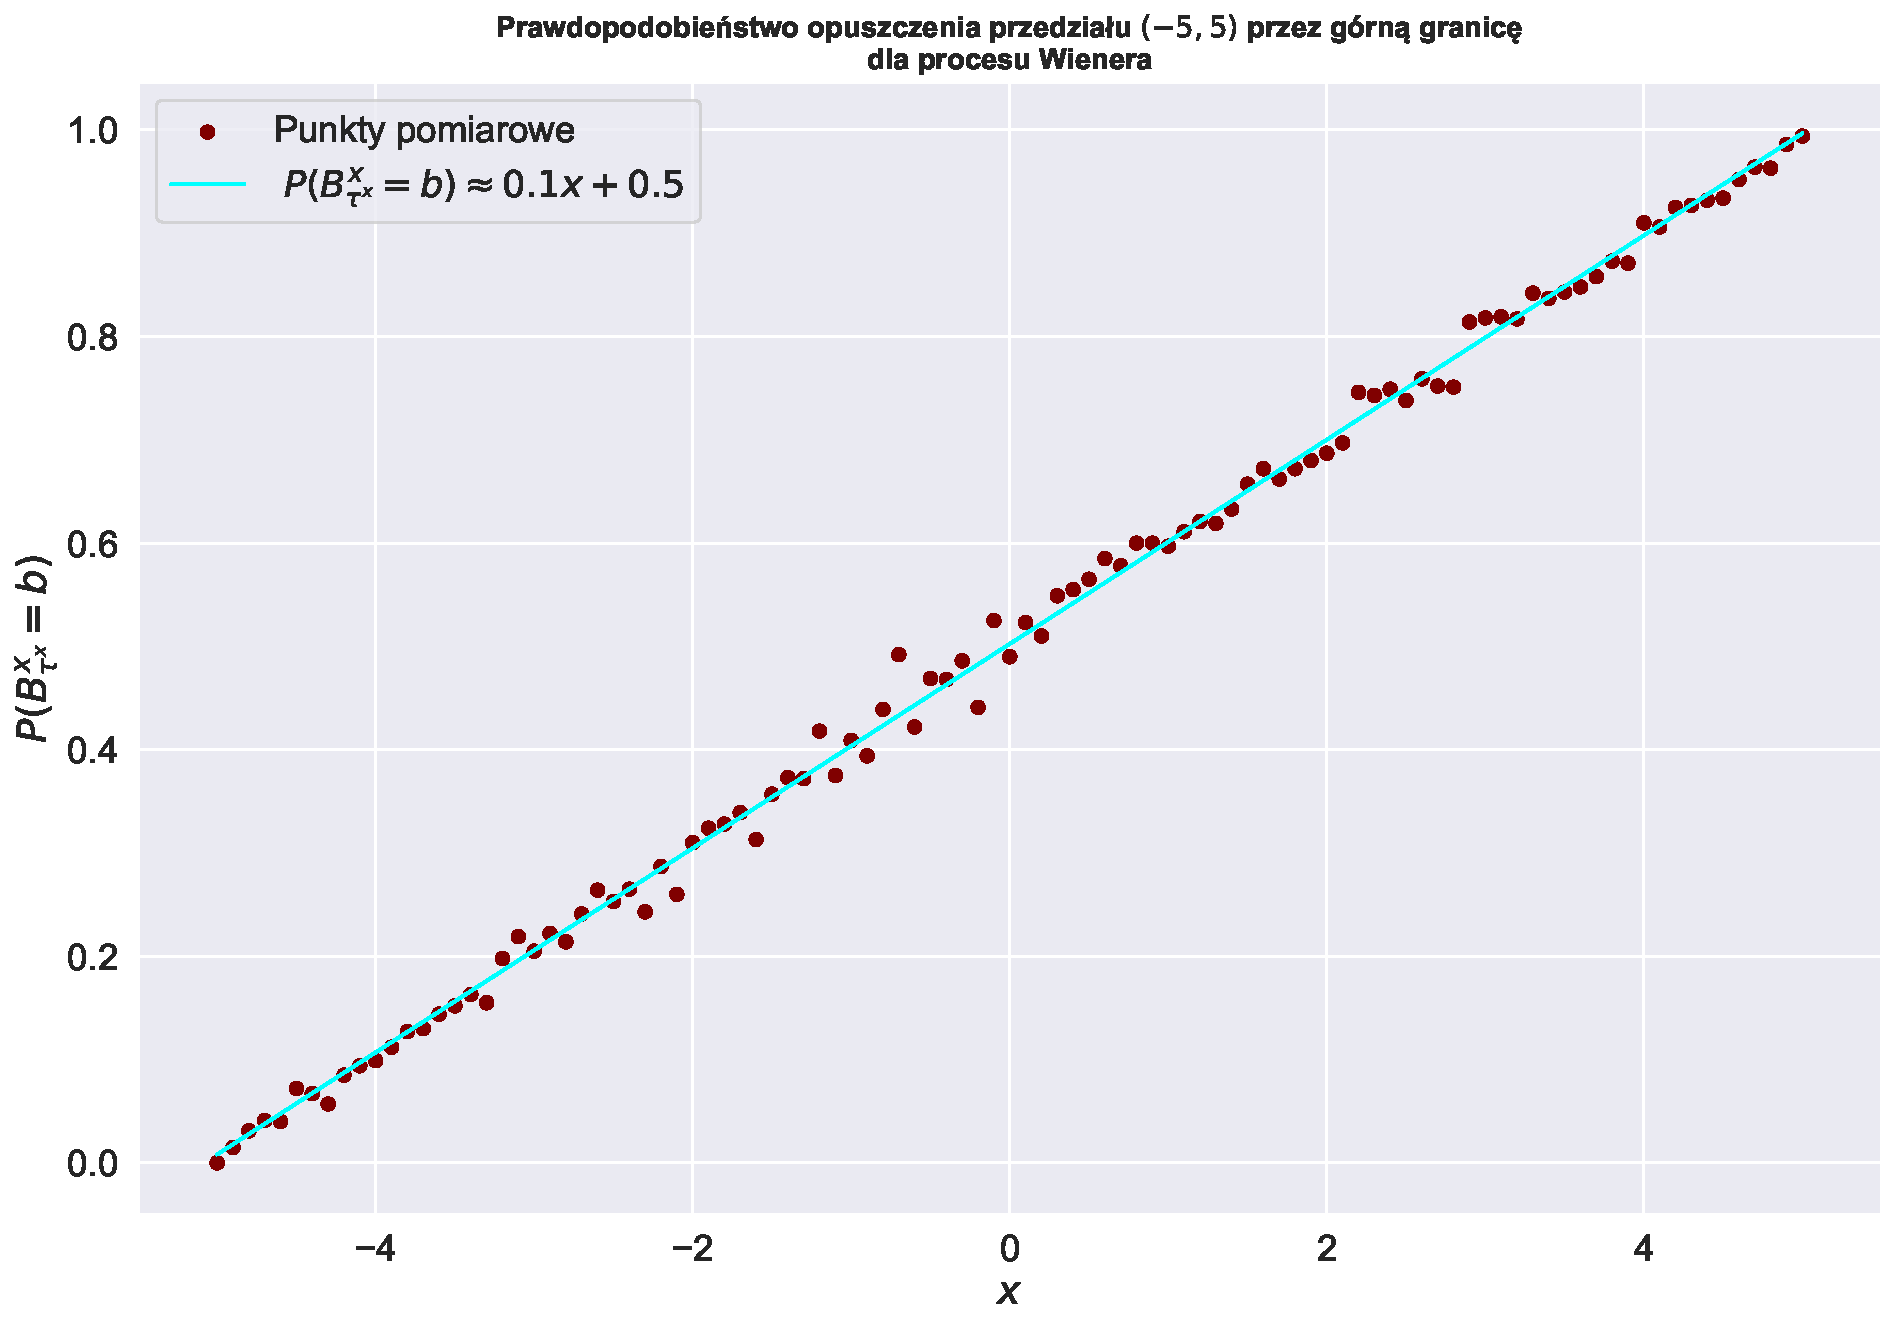
\includegraphics[scale=0.4]{2.pdf}
			\caption{Prawdopodobieństw wyjścia przez górną granicę dla zadanego przedziału przez proces Wienera wraz z krzywą dopasowania}
		\end{center}
	\end{figure}
\noindent Kształt przypomina zwykłą prostą i nie jest to dla nas zaskoczeniem, bazując na poprzednich wynikach. Możemy tutaj zobaczyć monotoniczność, bo bliska odległość do którejś z granic powoduje większe prawdopodobieństwo wyjścia przez nią. W momencie, gdy odległości $a = b$, to ich prawdopodobieństwa też są równe, co możemy zobaczyć w naszym przypadku.\\

 \subsection{Podsumowanie}
	\noindent W zadaniu drugim głównie korzystamy z własności procesu Wienera. Opis teoretyczny tego procesu pozwolił nam na dokładniejsze zrozumienie i wyznaczenie czasu opuszczenia przedziału oraz oszacowanie prawdopodobieństwa w momencie, gdy odbywa się to przez górną granicę.
	
	
\end{document} 